\documentclass{article}

\usepackage { fancyhdr } % headers and footers
\usepackage[headsep = 2.25cm, headheight = 0cm] { geometry } % showframe, margins
\usepackage { graphicx } % images
\usepackage[export] { adjustbox } % right or left for images
\usepackage[hidelinks] { hyperref } % hyperlinks
\usepackage { sectsty } % section font
\usepackage { array } % C macro
\usepackage { tikz }

\geometry {
    a4paper,
    total={180mm,220mm},
    left=20mm,
    top=30mm,
    bottom=30mm
}

\pagestyle{fancy}
\fancyhf{}
\renewcommand{\headrulewidth}{0pt} % no bottom border for header

% macro to center and wrap text in table cell
\newcolumntype{C}[1]{>{\centering\let\newline\\\arraybackslash\hspace{0pt}}m{#1}}
\newcolumntype{L}[1]{>{\raggedright\let\newline\\\arraybackslash\hspace{0pt}}m{#1}}

% font size of a section
\sectionfont{\fontsize{10}{15}\selectfont}

% header
\lhead { \small Bucharest,  \\ Romania  }
\chead { \textbf{ \Large Mihai-Bogdan Vîlculescu } }
\rhead { 
    \href{https://www.github.com/BogdanVM} {\includegraphics[width = .80cm, height = .80cm, right]{git2.png} }    
    \small email \\
    \small nr_telefon }

\lfoot { \href{https://www.linkedin.com/in/bogdan-vilculescu/} { \includegraphics[width = .80cm, height = .80cm, left]{linkedin.png} } }

% main document
\begin{document}
    
    % Experience Section
    \section*{ Experience }
        \setlength{\tabcolsep}{65pt}
        \begin{tabular} {ccL{3cm}}
            \footnotesize\textit{\textbf{Volunteer}} 
            & \footnotesize\textit{\textbf{Codette}} 
            & \footnotesize\textit{\textbf{March 2018 - Present}}\\
            \hline
        \end{tabular}

        \begin{itemize}
            \item \footnotesize Codette is a NGO having as an objective the empowerment of women to pursue careers in technology. As I empathize with the organisation's purpose, I joined in as a volunteer in March 2018, while in my first year at university. During this time, my involvement included mainly assistance with organizing different events, supported by Codette, such as the Code For All Summit in 2018.
        \end{itemize}

        \setlength{\tabcolsep}{20pt}
        \begin{tabular} {C{5cm}L{5cm}C{3cm}}
            \footnotesize\textit{\textbf{Tutor of Procedural Programming}} 
            & \footnotesize\textit{\textbf{University of Bucharest}} 
            & \footnotesize\textit{\textbf{November 2018 - January 2019}}\\
            \hline
        \end{tabular}

        \begin{itemize}
            \item \footnotesize Every year at my university, the student association organizes lessons for the first year students. The people who teach them are studying in the second year. In 2018, I participated as a tutor of procedural programming. This involved teaching C language concepts and mainly helping younger students understand this subject.
        \end{itemize}

        \setlength{\tabcolsep}{45pt}
        \begin{tabular} {ccC{3cm}}
            \footnotesize\textit{\textbf{Tutor of OOP}} 
            & \footnotesize\textit{\textbf{University of Bucharest}} 
            & \footnotesize\textit{\textbf{February 2019 - Present}}\\
            \hline
        \end{tabular}

        \begin{itemize}
            \item \footnotesize During the second semester in my second year, I held tutorials for the students at Object Oriented Programming. The subject involved the basic concepts of OOP (Encapsulation, Inheritance, Polymorphism), illustrated in C++.
        \end{itemize}

    % Education Section
    \section*{Education}
        \begin{tabular} {lC{6cm}L{3cm}}
            \footnotesize\textit{\textbf{BS Degree}} 
            & \footnotesize\textit{\textbf{Faculty of Mathematics and Informatics, University of Bucharest}} 
            & \footnotesize\textit{\textbf{October 2017 - June 2020}} (expected)\\
            \hline
        \end{tabular}

        \begin{itemize}
            \item \footnotesize Studied Algorithms, Programming Languages (C, C++, Java), Operating Systems, Web Technologies (Frontend).
        \end{itemize}

    % Personal Projects
    \section*{Personal Projects}
        \begin{itemize}
            \item \footnotesize \textbf{\textit{La Vot:}} This is an old project of mine developed around 2015 while I was still in high school. It was meant to be a platform where officials could administrate upcoming elections and citizens could use their right and vote online. I started working on it to get familiar with web technologies and this turned out to be my first full stack project. \textbf{Technologies used:} HTML, CSS, PHP and JavaScript.
            \item \textbf{\textit{BrioBAC:}} Created in 2017 during my last year at high school with a friend. It is a tool for high school students about to take the final exam at mathematics. It contains materials and tests to help with the understanding of the subject. There are 2 versions: PC and Android. \textbf{Technologies used (PC):} Visual C\#, SQL. \textbf{Technologies used (Android):} Java, XML, SQL, Php.
        \end{itemize}

    % Additional Experience Section
    \section*{Additional Experience}
        \begin{itemize}
            \item \footnotesize \textbf{\textit{Google Digital Workshop - Java Training (November 2018 - February 2019):}} Attended the workshop where I learnt the basic concepts of the Java language (Inheritance, Threads, Reactive, ...);
            \item \footnotesize \textbf{\textit{Google Digital Workshop - Android Advanced Training (March 2019 - Present)}};
            \item \textbf{\textit{Pedagogical Module(October 2018 - Present):}} Attended the pedagogical module held at our univeristy for people who wanted to become teachers. I do not necessarily intend to pursue a career in teaching, but I believe this is a great opportunity to learn and explore new things. 
        \end{itemize}
    
    % Languages and Technologies Section
    \section*{Languages and Technologies}
        \begin{itemize}
            \item[] \scriptsize 
                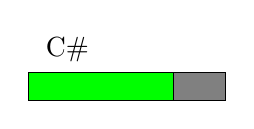
\begin{tikzpicture}
                    \node [anchor=west] at (.1,.65) {C\#};
                    \draw [fill=gray] (0,0) rectangle (2.5,.35);
                    \draw [fill={rgb:red,0;green,1;blue,0}] (0,0) rectangle (1.85, .35);
                \end{tikzpicture}
                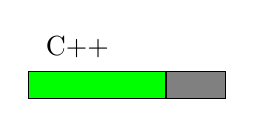
\begin{tikzpicture}
                    \node [anchor=west] at (.1,.65) {C++};
                    \draw [fill=gray] (0,0) rectangle (2.5,.35);
                    \draw [fill={rgb:red,0;green,1;blue,0}] (0,0) rectangle (1.75,.35);
                \end{tikzpicture}
                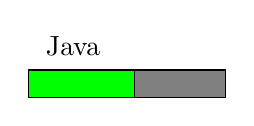
\begin{tikzpicture}
                    \node [anchor=west] at (.1,.65) {Java};
                    \draw [fill=gray] (0,0) rectangle (2.5,.35);
                    \draw [fill={rgb:red,0;green,1;blue,0}] (0,0) rectangle (1.35,.35);
                \end{tikzpicture}
                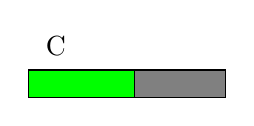
\begin{tikzpicture}
                    \node [anchor=west] at (.1,.65) {C};
                    \draw [fill=gray] (0,0) rectangle (2.5,.35);
                    \draw [fill={rgb:red,0;green,1;blue,0}] (0,0) rectangle (1.35,.35);
                \end{tikzpicture}
                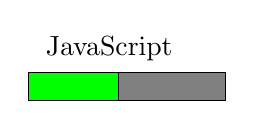
\begin{tikzpicture}
                    \node [anchor=west] at (.1,.65) {JavaScript};
                    \draw [fill=gray] (0,0) rectangle (2.5,.35);
                    \draw [fill={rgb:red,0;green,1;blue,0}] (0,0) rectangle (1.15,.35);
                \end{tikzpicture}
                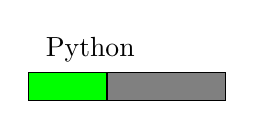
\begin{tikzpicture}
                    \node [anchor=west] at (.1,.65) {Python};
                    \draw [fill=gray] (0,0) rectangle (2.5,.35);
                    \draw [fill={rgb:red,0;green,1;blue,0}] (0,0) rectangle (1,.35);
                \end{tikzpicture}
            
            \item[]
                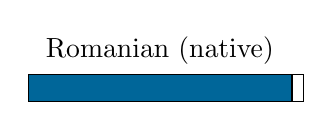
\begin{tikzpicture}
                    \node [anchor=west] at (.1,.65) {Romanian (native)};
                    \draw [fill=white] (0,0) rectangle (3.5,.35);
                    \draw [fill={rgb:red,0;green,2;blue,3}] (0,0) rectangle (3.35,.35);
                \end{tikzpicture}
                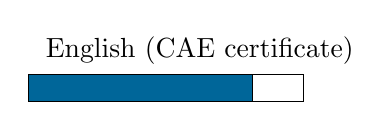
\begin{tikzpicture}
                    \node [anchor=west] at (.1,.65) {English (CAE certificate)};
                    \draw [fill=white] (0,0) rectangle (3.5,.35);
                    \draw [fill={rgb:red,0;green,2;blue,3}] (0,0) rectangle (2.85,.35);
                \end{tikzpicture}
                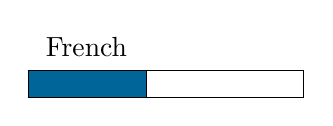
\begin{tikzpicture}
                    \node [anchor=west] at (.1,.65) {French};
                    \draw [fill=white] (0,0) rectangle (3.5,.35);
                    \draw [fill={rgb:red,0;green,2;blue,3}] (0,0) rectangle (1.5,.35);
                \end{tikzpicture}
            
        \end{itemize}
    
    % Hobbies and Interests Section
    \section*{Hobbies and Interests}
        \begin{itemize}
            \item \footnotesize Listening to music (heavy metal), Reading (science-fiction novels), Playing Strategy Games.
        \end{itemize}
\end{document}
